\documentclass[a4paper,papersize,dvipdfmx]{jsarticle}
\usepackage{ascmac}
\usepackage{mathtools, amssymb,bm}
\usepackage{comment}
\usepackage[hiresbb]{graphicx}
\usepackage{tcolorbox,color}
\usepackage{here}
\tcbuselibrary{raster,skins,breakable}

\newcommand{\pic}[1]{\begin{center} \includegraphics[width=1.0\linewidth,clip]{#1} \end{center}}   %写真用
\newcommand{\pict}[2]{\begin{center} \includegraphics[width= {#2} cm]{#1} \end{center}}   %写真用
\newcommand{\redunderline}[1]{\textcolor{red}{\underline{¥textcolor{black}{#1}}}}   %赤いアンダーライン
\newcommand{\mon}[1]{\item[({#1})] \ }
\newcommand{\ctext}[1]{\raise0.2ex\hbox{\textcircled{\scriptsize{#1}}}}%文字を丸囲みする(2桁の数字までならいける)

% 画像を貼る時はjpgかjpegで、pngはうまくいかないっぽい

%\itemを四角で囲った数字にする場合は以下のコメントアウトを消す
%\renewcommand{\labelenumi}{\textbf{\framebox[1.5zw]{\theenumi}}}


%enumerateの2階層めのカウンタを1,2,3, にする時は以下のコメントアウトを消す
\renewcommand{\theenumii}{\arabic{enumii}}

%enumerateのカウンタについては以下を参照
% http://www3.otani.ac.jp/fkdsemi/pLaTeX_manual/kajyo.html


%enumerateの番号の出力形式を変更するには、カウンタの値を出力する命令を定義し直す。
%レベル	カウンタ	出力する命令	デフォルトの出力
%1	enumi	¥theenumi	アラビア数字(1,2,3,・・・)
%2	enumii	¥theenumii	小文字のアルファベット(a,b,c,・・・)
%3	enumiii	¥theenumiii	小文字のローマ数字(小文字のローマ数字(\UTF{2170},\UTF{2171},\UTF{2172},・・・)
%4	enumiv	¥theenumiv	大文字のアルファベット(A,B,C,・・・)
%例:¥enumiカウンタを大文字のローマ数字で出力する設定
% ¥renewcommand{¥theenumi}{¥Roman{enumi}}

% 番号の出力形式
%命令	出力形式
%¥arabic	アラビア数字(1、2、3、・・・)
%¥roman	ローマ数字(\UTF{2170}、\UTF{2171}、\UTF{2172}、・・・)
%¥Roman	ローマ数字(\UTF{2160}、\UTF{2161}、\UTF{2162}、・・・)
%¥alph	アルファベット(a、b、c、・・・)
%¥Alph	アルファベット(A、B、C、・・・)




\begin{document}

\title{実習レポート 薬品代謝化学教室}
\author{10191043 鈴木健一}
%作成日を入れる場合は消す
\date{}
\maketitle

%以下の3つからフォントサイズを選択するとよい
%\footnotesize
%\small
%\normalsize


\begin{flushright}
実習班 : 11班 

実験日 : 2019/6/18 $\sim$ 2019/6/24
\end{flushright}

\part*{実験1 薬物代謝反応}

\section*{目的}
代謝研究の基礎としてラット肝のミクロゾーム分画を用いた$in \ vitro$での代謝反応を中心に実験を行うことにより、代謝薬物について学ぶ。

\section*{1日目 - 実験方法}

\subsection*{誘導、および肝ミクロゾーム調整(ビデオ)}
\begin{enumerate}
\item ラットにβ−naphthoflavone を経口投与
\item 麻酔であるソムノペンチルを投与する
\item 腹膜を切開
\item 正中線を切開
\item 横に切り開く
\item 腸管をどかす
\item 脂肪成分を取り除くと下行大静脈が出てくるので1.1%塩化カリウム溶液を注入する。
\item 肝臓が大きく膨らむので揉みほぐす。これを4回行う。
\item 肝臓を切除する
\item 肝臓を塩化カリウム溶液で洗浄する
\item 氷上に置く
\item 肝臓の4倍量のバッファーを加え、ホモジェナイザーですり潰す
\item 綺麗にすり潰せなかった組織を取り除くために遠心分離する
\item 超遠心装置で80分間遠心する
\item 上澄みを捨てるとミクロソームのペレットが得られる
\item 重量を測る
\item マイナス80度で保存する

\end{enumerate}
\subsection*{タンパク質含量の測定}
\begin{enumerate}
\item 4\%硫酸銅水溶液0.20 mLをBCA溶液10 mLに加え、vortexミキサーを用いてすぐによくかき混ぜる。
\item BSA 200 μg/mL 溶液を試験管中で順次希釈して、BSA 25,50,100,150 μg/mL の各溶液 2.0 mLずつを調整する。
\item 検量線測定用に、BSA 200 μg/mL 溶液、(2)で作成した各濃度のBSA溶液をそれぞれ50 μLずつ別の試験管に加える。またブランクとして50 μLを別の試験管に加える。そして、これらと同様に、ミクロゾーム希釈液を別の試験管に加える。
\item 1.で調整した試薬1 mLを各試験管に加えてよく混合する。
\item 口をアルミホイルで覆い、インキュベータで37℃、30分インキュベートする。
\item 混合液を室温まで冷やし、混合液全量に蒸留水3.0 mLを加え、希釈する。
\item 吸光光度計にて各サンプル希釈液の562 nm吸収の吸光度を測定する。
\item BSA溶液の吸光度から検量線を作成し、ミクロゾームのタンパク質含量を求める。肝ミクロゾームのタンパク質含量は3本作った試験管の平均をとって算出する。

\end{enumerate}
\subsection*{cytochrome P450 含量の測定}
\begin{enumerate}
\item 0.1 M Tris-HCl buffer 5.5 mL を50 mL三角コルベンに入れる。そこに、0.50 mLの肝ミクロゾーム希釈液を加えて混ぜる。
\item 溶液が均一になったら、分光セル2つにほぼ均一に分ける。
\item 2つの分光セルを分光計のsample 側と reference 側にに入れベースライン補正を行う。この際サンプルが冷たいと曇りを生じてデータがぶれやすいので、サンプルは氷浴から出して室温近辺に戻してから測定を行う。
\item 両方のセルを取り出し、sample 側のセルにCOガスを約1分間バブルする。その直後、両方のセルにミクロスパーテルで半分ほどの$\rm Na_2S_2O_4$を加える。パラフィルムでセルの口をふさぎ、数回ゆっくりと転倒混和を行った後、両方のセルを分光計に戻し、差スペクトルを測定する。
\item $\rm A_{450} - A_{490}$からP450のミクロゾーム mg protein あたりの濃度を計算する。

\end{enumerate}
\section*{結果}
\begin{enumerate}
\item 吸光光度計にて各サンプル希釈液の562 nm吸収の吸光度を測定した結果

\begin{table}[H]
\begin{center}
\begin{tabular}{|c|c|c|c|c|c|c|}
\hline
BSA concentration (μg/mL) & 0     & 25    & 50    & 100   & 150  & 200   \\ \hline
Absorbance                & 0.034 & 0.044 & 0.055 & 0.073 & 0.09 & 0.105 \\ \hline
\end{tabular}
\end{center}
\end{table}

\pict{imgs/day1-1.png}{8}

\item ミクロゾームのタンパク質含量

\begin{table}[H]
\begin{center}
\begin{tabular}{|c|c|c|c|}
\hline
平均値    & サンプル1    & サンプル2    & サンプル3    \\ \hline
0.0727 & 0.073 & 0.073 & 0.072 \\ \hline
\end{tabular}
\end{center}
\end{table}



検量線の傾きをもとに肝ミクロゾームのタンパク質含有量を求めると以下のようになる。

\[\frac{(7.27 \cdot 10^{-2} -3.57 \cdot 10^{-2})}{3.56 \cdot 10^{-4}} \times 800 = 8.31 \cdot 10^{4} \ [\rm{μg/mL}] = 83.1 \ [\rm{xg/mL}]\]


\item 差スペクトル$\rm A_{450} - A_{490}$からP450のミクロゾーム mg protein あたりの濃度を計算する。

\begin{table}[H]
\begin{center}
\begin{tabular}{|c|c|c|}
\hline
$\Delta A$     & $\epsilon$  & c/60 (mM)          \\ \hline
0.136 & 91 & $1.49 \cdot 10^{-3}$ \\ \hline
\end{tabular}
\end{center}
\end{table}

表より60倍に希釈されたP450の濃度が$1.49 \cdot 10^{-3}$であるから、P450の肝ミクロゾーム mg protein あたりの濃度は以下のようにして求められる。このとき、上で求めた肝ミクロゾームのタンパク質濃度を用いる。

\[1.49 \cdot 10^{-3} \times 60 \times 10^{3} \div 83.1 = 1.08 \  [\rm nmol/mg  \ protein]\]

\end{enumerate}
\section*{2日目 - 実験方法}
\subsection*{7-Ethoxycoumarin の$O$-脱エチル化反応}
non-treat群(non)、フェノバルビタール投与群(PB)、β-ナフトフラボン投与群(NF)、のラット肝ミクロゾームを用いて以下の反応を行う。

\pict{imgs/image1.png}{8}

蛍光物質である生成物のウンベリフェロンの蛍光強度を測定する。PB群についてはP450特異的な阻害剤のシメチジンを添加したものの反応もあわせて行った。

反応に必要なすべての試薬を加えるcomplete系(SM)、酵素を加えないSubstrate Blank系(SB)、基質を入れずに反応を行い反応後、後処理前に生成物を添加するStandard系(ST)、阻害剤シメチジンを加えるPB群のIN系で計8本の試験管について反応を行う。緩衝液、NADPH生成系、ミクロゾーム希釈液を試験管で混合し、37℃、5分間のpre-incubationののち、基質の50mM 7-エトキシクマリンMeOH溶液を10uL加え、37℃、15分incubationし、10分氷冷後、遠心分離(3000rpm,10min)し、上清1.0mLをリン酸カリウム緩衝液で希釈し蛍光測定した。STのウンベリフェロンはインキュベーション後に0.5mMを0.2mL(100 nmol)加えている。

\section*{結果}

Ex. 380 nm、Em. 460 nmで測定された蛍光強度は以下の通りである。

\begin{table}[H]
\begin{center}
\begin{tabular}{|c|c|c|c|c|c|c|c|c|}
\hline
種類   & SB    & IN(NF) & SM(non) & SM(PB) & SM(NF) & ST(non) & ST(PB) & ST(NF) \\ \hline
蛍光強度 & 60.45 & 4014   & 1065    & 836.9  & 4874   & 3558    & 3382   & 3227   \\ \hline
\end{tabular}
\end{center}
\end{table}

\

またミクロゾームのタンパク質濃度とタンパク質あたりのP450含量の値は、以下のようになる。

\begin{table}[H]
\begin{center}
\begin{tabular}{|c|c|c|}
\hline
& タンパク質含量(mg protain/mL) & P450含量(nmol P450/mg protain)  \\ \hline
non                    & 51.0              & 0.818       \\ \hline
PB                     & 83.1              & 1.08 		\\ \hline
NF                     & 67.1               & 0.798       \\ \hline
\end{tabular}
\end{center}
\end{table}

この値と以下の式からタンパク質あたりの$O$-脱エチル化活性、およびP450あたりの$O$-脱エチル化活性が求まる。

\[\rm{Activity} = \frac{F_{SM}-F_{SB}}{F_{ST}-F_{SB}} \times \frac{100}{15} \div \rm{Amount \ of \ protein}\]

\begin{table}[H]
\begin{center}
\begin{tabular}{|c|c|c|}
\hline
& タンパク質あたりの活性 & P450あたりの活性     \\ \hline
non       & 0.6        & 0.703 \\ \hline
PB        & 0.3        & 0.266  \\ \hline
NF        & 2.3        & 2.902   \\ \hline
\end{tabular}
\end{center}
\end{table}

\section*{課題}
\begin{tcolorbox}[colback=white,colbacktitle=black!10!white,coltitle=black,title={(1)}]
誘導、非誘導ミクロゾームによる 7-ethoxycoumarin の$O$-脱エチル化および aminopyrine の$N$-脱メチル化反応のそれぞれの反応効率の違いを比較し、パターンの相違およびP450分子種との関連について考察せよ。
\end{tcolorbox}

実習書の参考実験によると、aminopyrine の$N$-脱メチル化活性は以下のような結果となる。

\begin{table}[H]
\begin{center}
\begin{tabular}{|c|c|c|}
\hline
& タンパク質あたりの活性  & P450あたりの活性    \\ \hline
non & 4.61       & 5.54 \\ \hline
PB  & 6.22       & 4.14 \\ \hline
NF  & 4.82       & 5.63 \\ \hline
\end{tabular}
\end{center}
\end{table}


ミクロゾームのタンパク質1 mgあたりの代謝活性はnon treat群に比べてフェノバルビタール投与群では著しく上昇しているのに対し、$\beta -$ナフトフラボン投与群の上昇値は小さい。このことからフェノバルビタールが誘導するCYP2Bはアミノピリン代謝に関わっているが、$\beta -$ナフトフラボンが誘導するCYP1A1は代謝に関わっていないことが分かる。
P450あたりの活性ではフェノバルビタール投与群も$\beta -$ナフトフラボン投与群も共にnon treat群に比べて減少している。これはフェノバルビタールがアミノピリン代謝に有効なP450分子種だけでなくアミノピリン代謝に関与しないP450分子種も誘導するために、全体としてP450あたりのアミノピリン代謝活性が低くなっていると考えられる。

一方、実習の結果を元に7-ethoxycoumarin のタンパク質あたりの$O$-脱エチル化活性について考察すると、non treat群に比べてフェノバルビタール投与群は低下しているが、$\beta -$ナフトフラボン投与群は著しく上昇している。
さらに、P450あたりの活性でも同様にnon treat群に比べて、フェノバルビタール投与群では減少、$\beta -$ナフトフラボン投与群では著しく上昇している。このことから、フェノバルビタールが誘導するP450分子種は7-ethoxycoumarinの代謝には無関係であり、$\beta -$ナフトフラボンで誘導されるCYP1A1が7-ethoxycoumarinの代謝に大きく寄与していることが分かる。

\begin{tcolorbox}[colback=white,colbacktitle=black,coltitle=white,title={(2)}]
P450含量の測定の際、450nmにおけるスペクトルの差の吸光度からP450含量が求められる理由を考察せよ。
\end{tcolorbox}

P450はCO配位で450 nmに特有の吸光を持っているが、P450以外の肝ミクロゾームにもヘム中心のCOが配位することによって450nmの光を吸光するタンパク質が存在する。そのP450以外の450 nmの吸光の影響を排除するために、吸光に差がないとされる490 nmでの吸光を450 nmでの吸光度から引くことでP450による吸光度を求めることができる。

\begin{tcolorbox}[colback=white,colbacktitle=black,coltitle=white,title={(3)}]
P450阻害作用のある薬物の一例として cimetidine を用いたが、この構造のどの部分が阻害作用に効率的であったか考察せよ。実習書のFigure6でのcimetidine添加によるミクロゾームの吸光スペクトル変化との関連についても記すこと。また他の薬物でも構造上P450阻害が予想される例を一つあげよ。
\end{tcolorbox}

P450はアゾール環をもつ薬物によって阻害される。cimetidinもアゾール環をもつためP450Wを阻害すると考えられる。これはアゾール環のN上の非共有電子対がP450中心のヘム鉄に競合的に配位結合を形成して、基質の7-ethoxycoumarinとの結合を阻害しているからである。

Figure 6.によるとcimetidin添加時の吸収差スペクトルは428 nm付近で最大となっている。これはcimetidinのアゾール環のNがcimetidinに配位することでヘム鉄の吸光スペクトルが変化したからだと考えられる。

cimetidin以外でP450を阻害する薬物としては、ケトコナゾールが挙げられる。これも同様にアゾール環をもつ。

\part*{実験2 酵素反応解析法と蛍光プローブを用いた実験}

\section*{目的}
酵素反応の速度論的ファクターおよび各種プロットの質的意味を理解する。また、蛍光プローブの原理や操作について理解する。

\section*{実験方法および結果}
\subsection*{蛍光プローブを用いた実験の基礎}

\subsubsection*{各種pHでの2-Me-4 OMe-TGのスペクトル測定}

1mM 2-Me-4-OMe-TGのDMSO溶液をpH 4.0,7.4,11.0のナトリウムリン酸緩衝液で1000倍に希釈し、蛍光強度と吸光度を測定する。結果のスペクトル図はレポートに添付している。

\subsubsection*{考察}

吸光度についても蛍光強度についてもpH4.0のスペクトルはPH 7.4,pH11.0のスペクトルと大きく異なる。

pH4.0のスペクトルは430 nm付近で最大吸収波長を持ち、492 nmで最大蛍光波長を持つ。一方pH7.4とpH11.0では492 nm付近に最大吸収波長を持ち、510 nm付近に最大蛍光波長を持つ。また、pHによって最大蛍光波長の蛍光強度も大きく異なる。pH4.0では10にも満たないのに対し、pH7.4では500、pH11.0では115にもなる。よってpH4.0でのスペクトルはレイリー散乱を表していると考えられる。このようにpHによってスペクトルの形状が大きく異なるのは2-Me-4-OMe-TGがアニオンの状態では蛍光を持つが、pHが低くプロトン化された状態では蛍光を持たないからであると考えられる。2-Me-4 OMe-TGの蛍光団の-OHのpKaは6.4であることを元に計算すると、pH 4.0では分子形がアニオンに比べて102.4倍ほど多くなる。一方、pH 7.4ではアニオンが分子型の10倍ほど、pH 11.0ではアニオンが分子形の103.6倍となる。しかし、理論値とは対照的にpH7.4の方がpH11.0よりも蛍光強度が強かった。これは共洗いなどで液が混ざってしまったことや、セル内の濃度が均一でなかったなどの要因が考えられる。


\subsubsection*{TG-βGalによるβ-galactosidase活性の検出}

pH 7.4ナトリウムリン酸緩衝液で1mM TG-βGalのDMSO溶液を1000倍に希釈したものを2本用意し、片方にβ-galactosidaseを入れて調整する。10分経過後に両サンプルの吸収・蛍光スペクトルを計測する。計測結果のスペクトルはレポートに添付している。

\subsubsection*{考察}
β-galactosidaseを入れた方のサンプルで492 nm付近に最大吸収波長が見られた。一方β-galactosidaseを入れなかった方のサンプルではTG-βGalによって530 nm付近に最大吸収波長が見られた。また、蛍光強度もβ-galactosidaseを入れた方のサンプルでは2-Me-4-OMe-TGのpH7.4やpH11の時と同じようなスペクトルを得られた。β-galactosidaseを入れなかった方ではpH4.0の時のようなスペクトルを得られた。これは実習書にもあるようにTG-βGalにβ-galactosidaseが作用するとアニオンの状態の2-Me-4-OMe-TGが得られるため、電子の励起状態が蛍光によって解消することが可能になるからである。

\subsection*{酵素反応速度論解析}

\subsubsection*{吸光度の計測}
TG-βGalを基質として濃度が1, 5, 10, 25, 50, 100 $\mu$Mになるよう緩衝液で調整し、$\beta$-galactosidaseを$4.0 \times 10^{-6}$ $\mu$Mとなるように加えて、加えてから時刻0, 10, 20, 30, 40, 50, 60, 70 (sec)で吸光度を測る。測定結果は以下のようになった。

\begin{table}[H]
\begin{center}
\begin{tabular}{|c|c|c|c|c|c|c|c|c|}
\hline
Time(sec) & 0     & 10    & 20    & 30    & 40    & 50    & 60    & 70    \\ \hline
\#1       & 0.006 & 0.007 & 0.008 & 0.009 & 0.009 & 0.010 & 0.010 & 0.010 \\ \hline
\#2       & 0.037 & 0.039 & 0.041 & 0.044 & 0.047 & 0.049 & 0.050 & 0.053 \\ \hline
\#3       & 0.130 & 0.136 & 0.142 & 0.149 & 0.156 & 0.164 & 0.170 & 0.177 \\ \hline
\#4       & 0.334 & 0.347 & 0.361 & 0.375 & 0.388 & 0.401 & 0.415 & 0.428 \\ \hline
\#5       & 0.611 & 0.621 & 0.635 & 0.648 & 0.659 & 0.671 & 0.676 & 0.687 \\ \hline
\#6       & 0.721 & 0.739 & 0.756 & 0.771 & 0.785 & 0.810 & 0.841 & 0.841 \\ \hline
\end{tabular}
\end{center}
\end{table}

\pict{imgs/Absorbance.png}{12}


これ以降の解析についてはコンピュータを用いて行う。実習で用意されたExcelのプログラムとは別に、独自に開発したプログラム(https://github.com/utp2018th/plot-graph/tree/finish-all)でもプロットをしているので両者のデータを見ていきたいと思う。

グラフに表示されている検量線の傾き$\Delta A$を元に反応速度を求める。
さらに反応速度と基質濃度のデータから

\begin{enumerate}
\item Michaelis-Menten (6 dots)
\item Michaelis-Menten (4 dots)
\item Lineweaver-Burk
\item Eadie-Hofstee
\end{enumerate}

の4種類のプロットを行う。

\newpage

\subsubsection*{1. Michaelis-Menten (6 dots)}
以下のMichaelis-Menten式に従うように最小二乗法で$V_{max}$と$K_m$をパラメータとして非線形最小二乗法プログラムで最適化した。
\[v=\frac{V_{max} *[S] }{K_m + [S]}\]

\begin{figure}[H]
\begin{center}
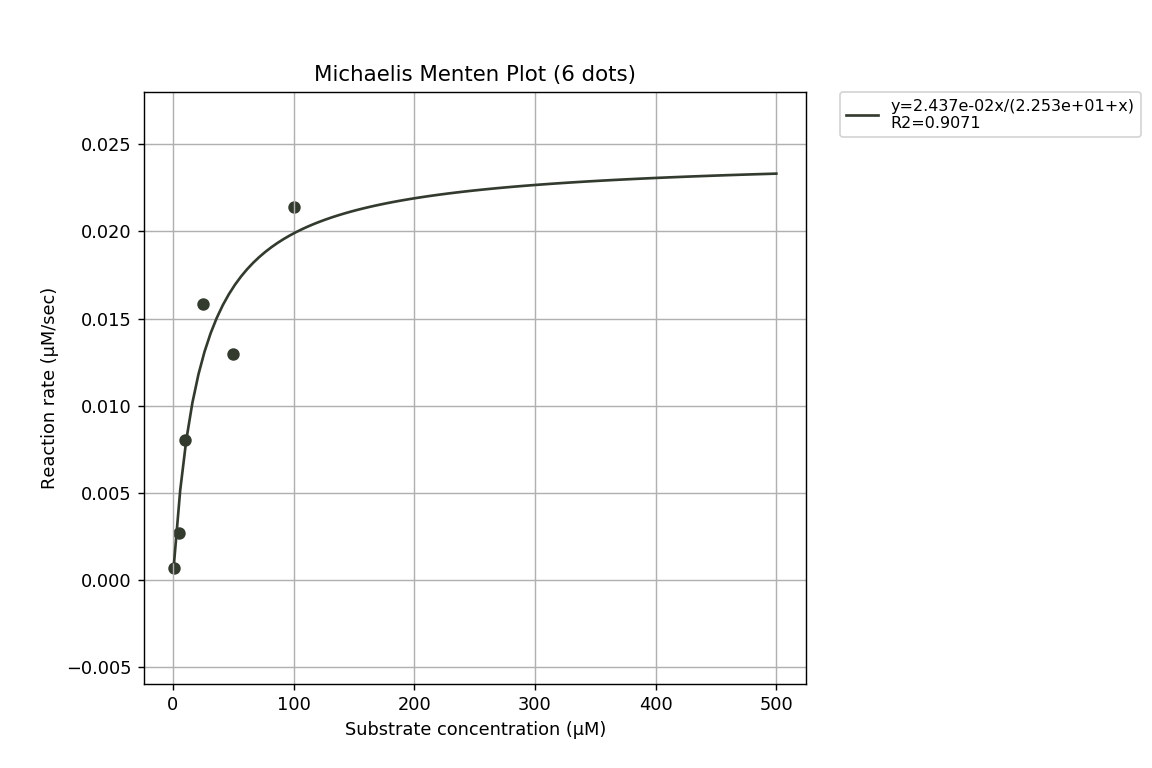
\includegraphics[clip, height=7cm]{imgs/MichaelisMenten6.png}
\caption{M-M plot6 (自作)}
\end{center}
\end{figure}

\begin{figure}[H]
\begin{center}
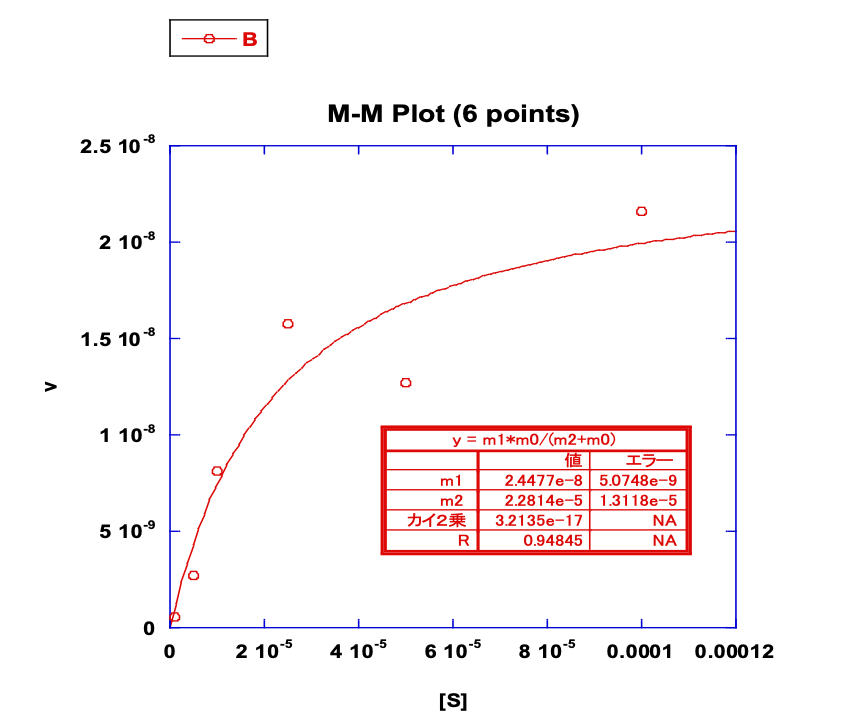
\includegraphics[clip, height=7cm]{imgs/11-mm6.png}
\caption{M-M plot6 (実習)}
\end{center}
\end{figure}


\subsubsection*{2.  Michaelis-Menten (4 dots)}
1と同じようにMichaelis-Menten式に従うように最適化をしているが、基質濃度が酵素が飽和する状態に達してい無いデータで最適化をしているため、1番のグラフと比べて高濃度領域での誤差が大きくなっていることが分かる。

\begin{figure}[H]
\begin{center}
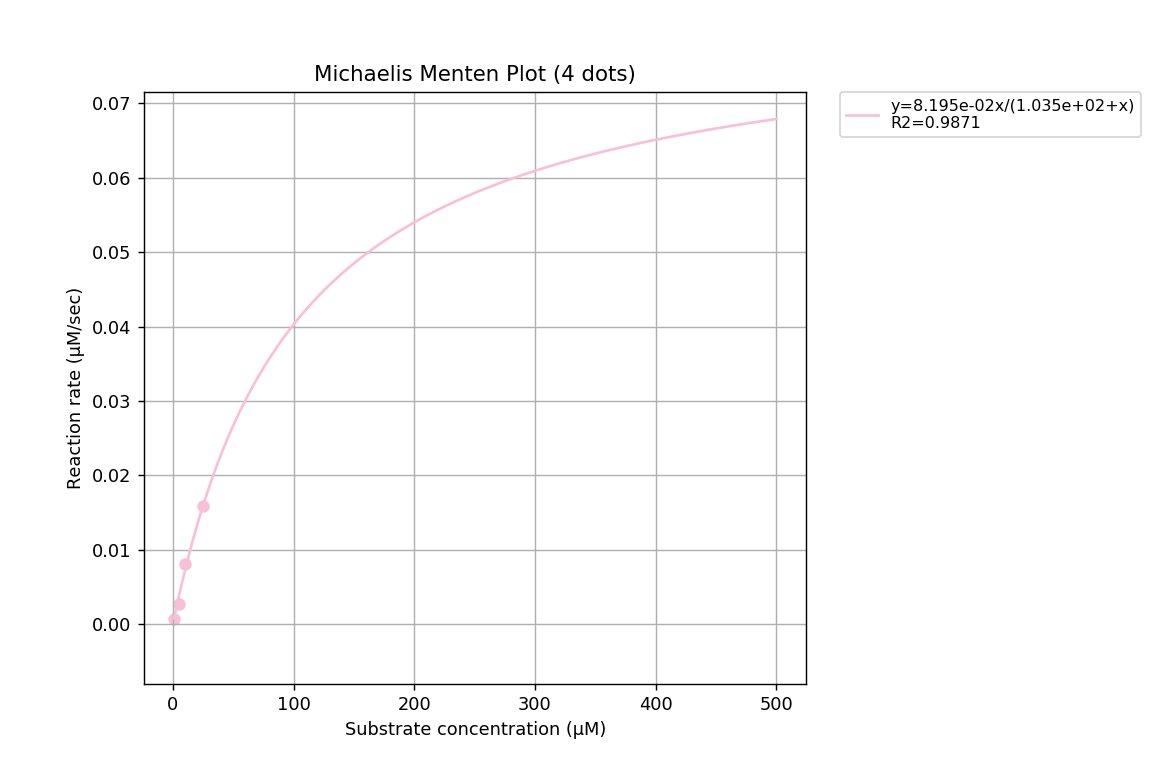
\includegraphics[clip, height=7cm]{imgs/MichaelisMenten4.png}
\caption{M-M plot4 (自作)}
\end{center}
\end{figure}

\begin{figure}[H]
\begin{center}
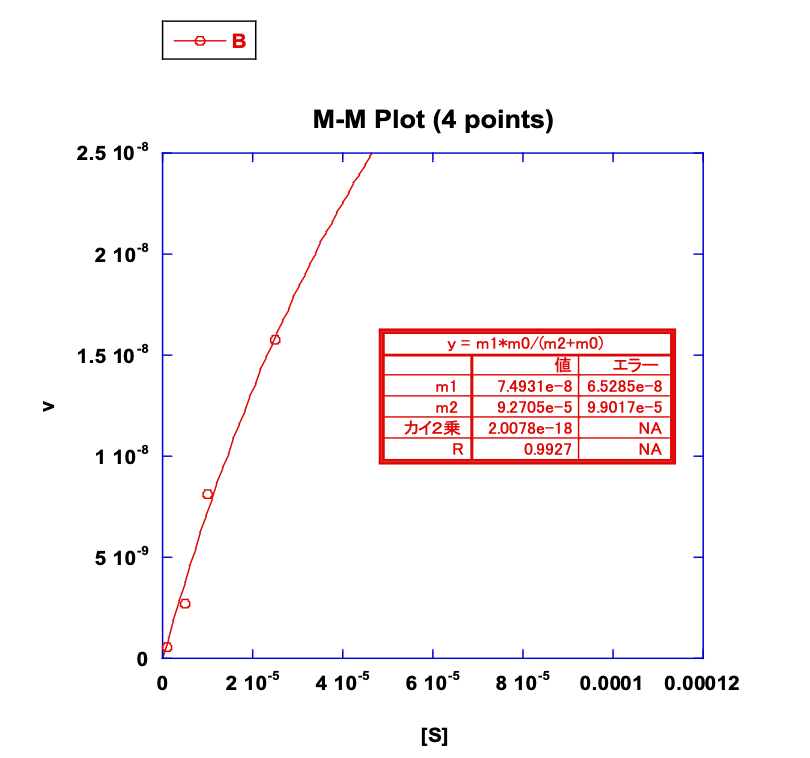
\includegraphics[clip, height=7cm]{imgs/11-mm4.png}
\caption{M-M plot4 (実習)}
\end{center}
\end{figure}


\subsubsection*{3. Lineweaver-Burk}
\[\frac{1}{v} = \frac{1}{V_{max}}+\frac{K_m}{V_{max}*[S]}\]
となるような逆数プロットである。

\begin{figure}[H]
\begin{center}
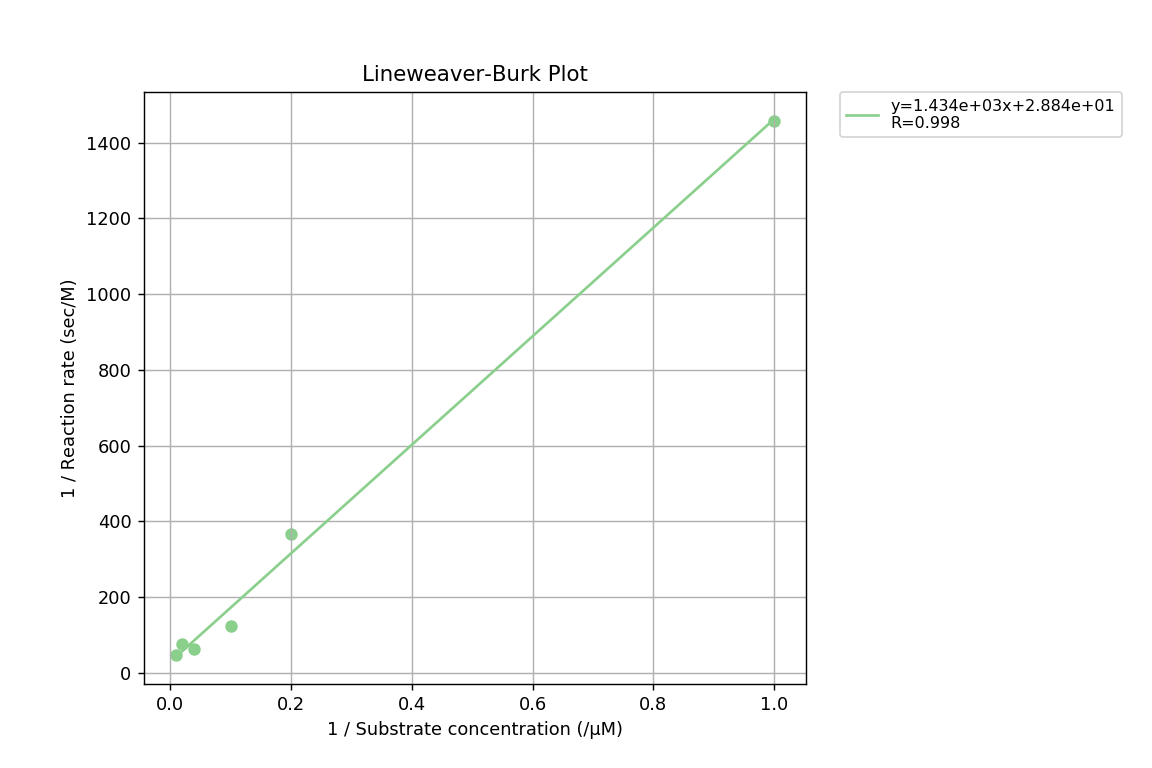
\includegraphics[clip, height=7cm]{imgs/Lineweaver-Burk.png}
\caption{L-B plot (自作)}
\end{center}
\end{figure}

\begin{figure}[H]
\begin{center}
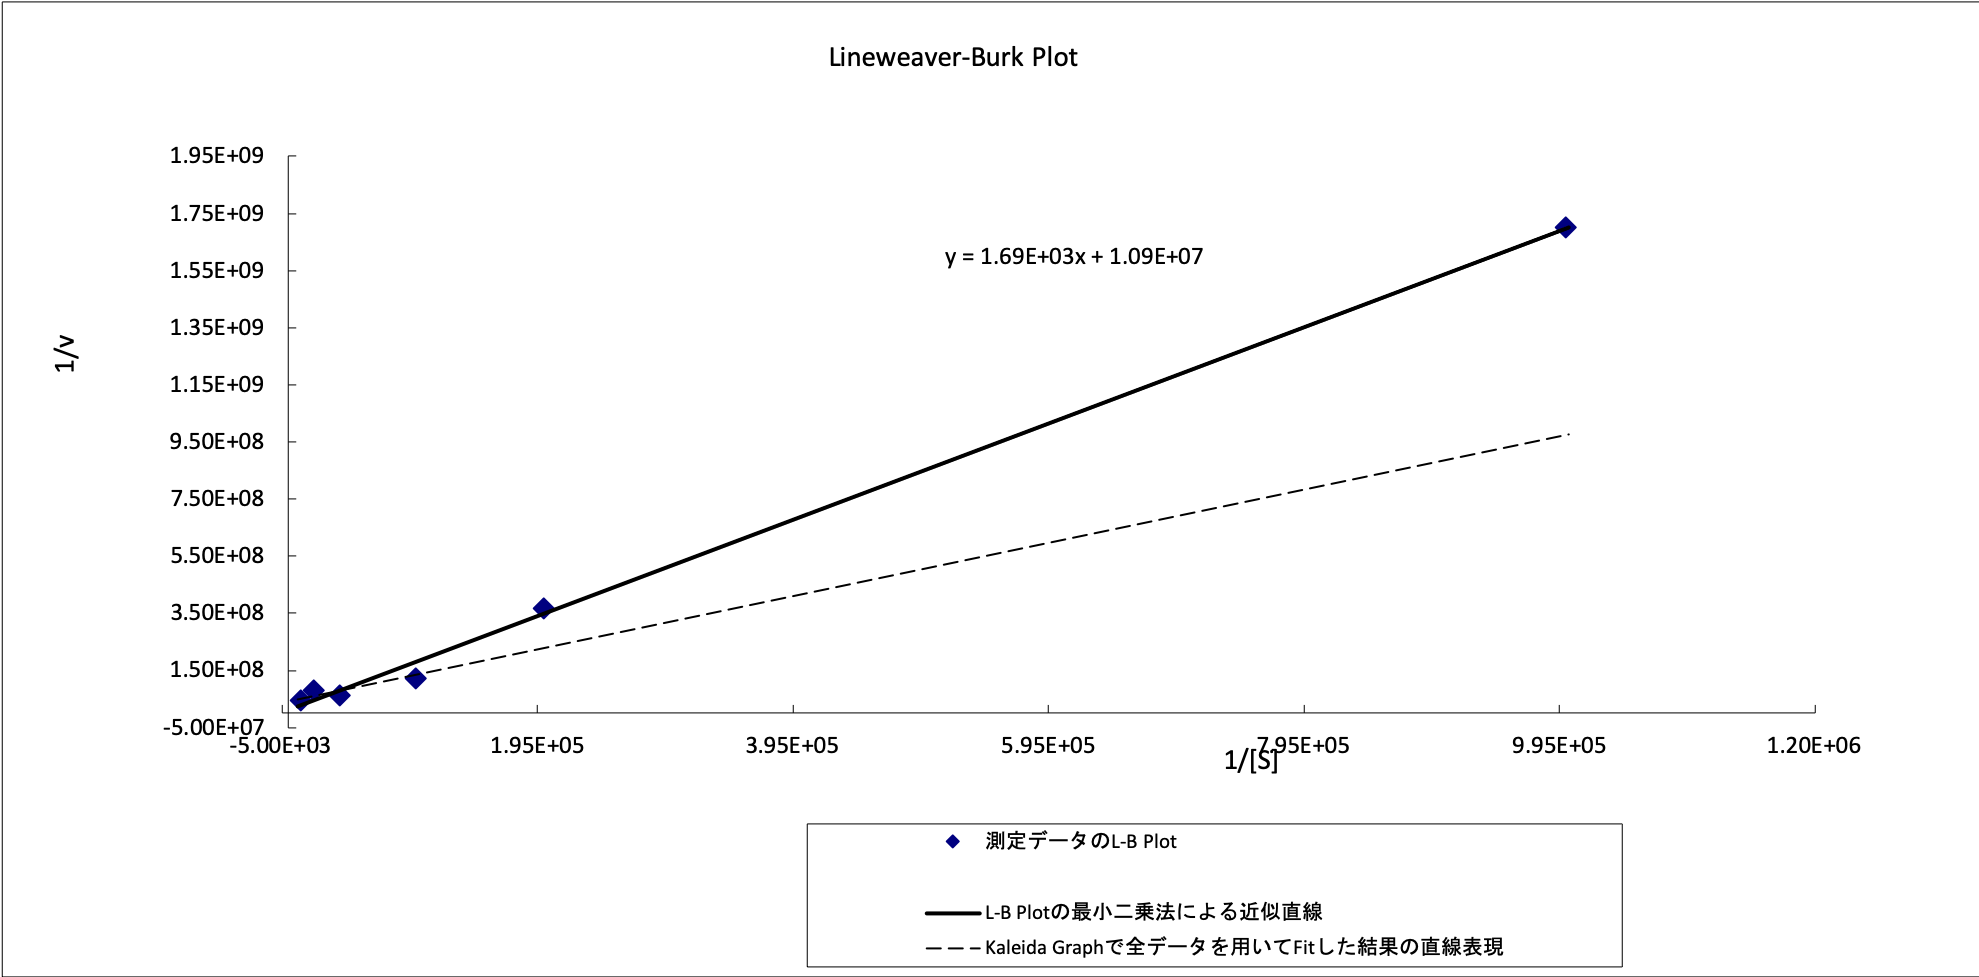
\includegraphics[clip, height=7cm]{imgs/11-lb.png}
\caption{L-B plot (実習)}
\end{center}
\end{figure}

\subsubsection*{4. Eadie-Hofstee}
Lineweaver-Burkの式を改良したものである。横軸に$v/[S]$、縦軸に$v$をプロットする。
\[v = V_{max} - \frac{K_m * v}{[S]}\]

\begin{figure}[H]
\begin{center}
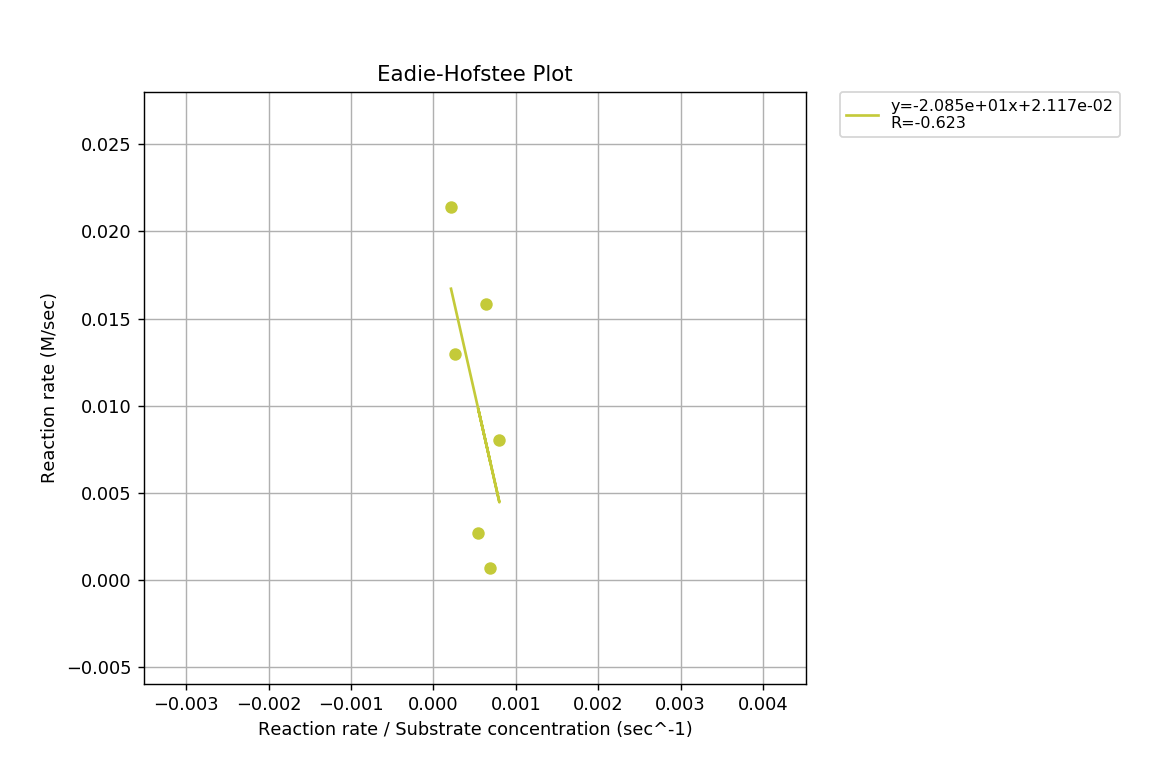
\includegraphics[clip, height=7cm]{imgs/Eadie-Hofstee.png}
\caption{E-H plot (自作)}
\end{center}
\end{figure}

\begin{figure}[H]
\begin{center}
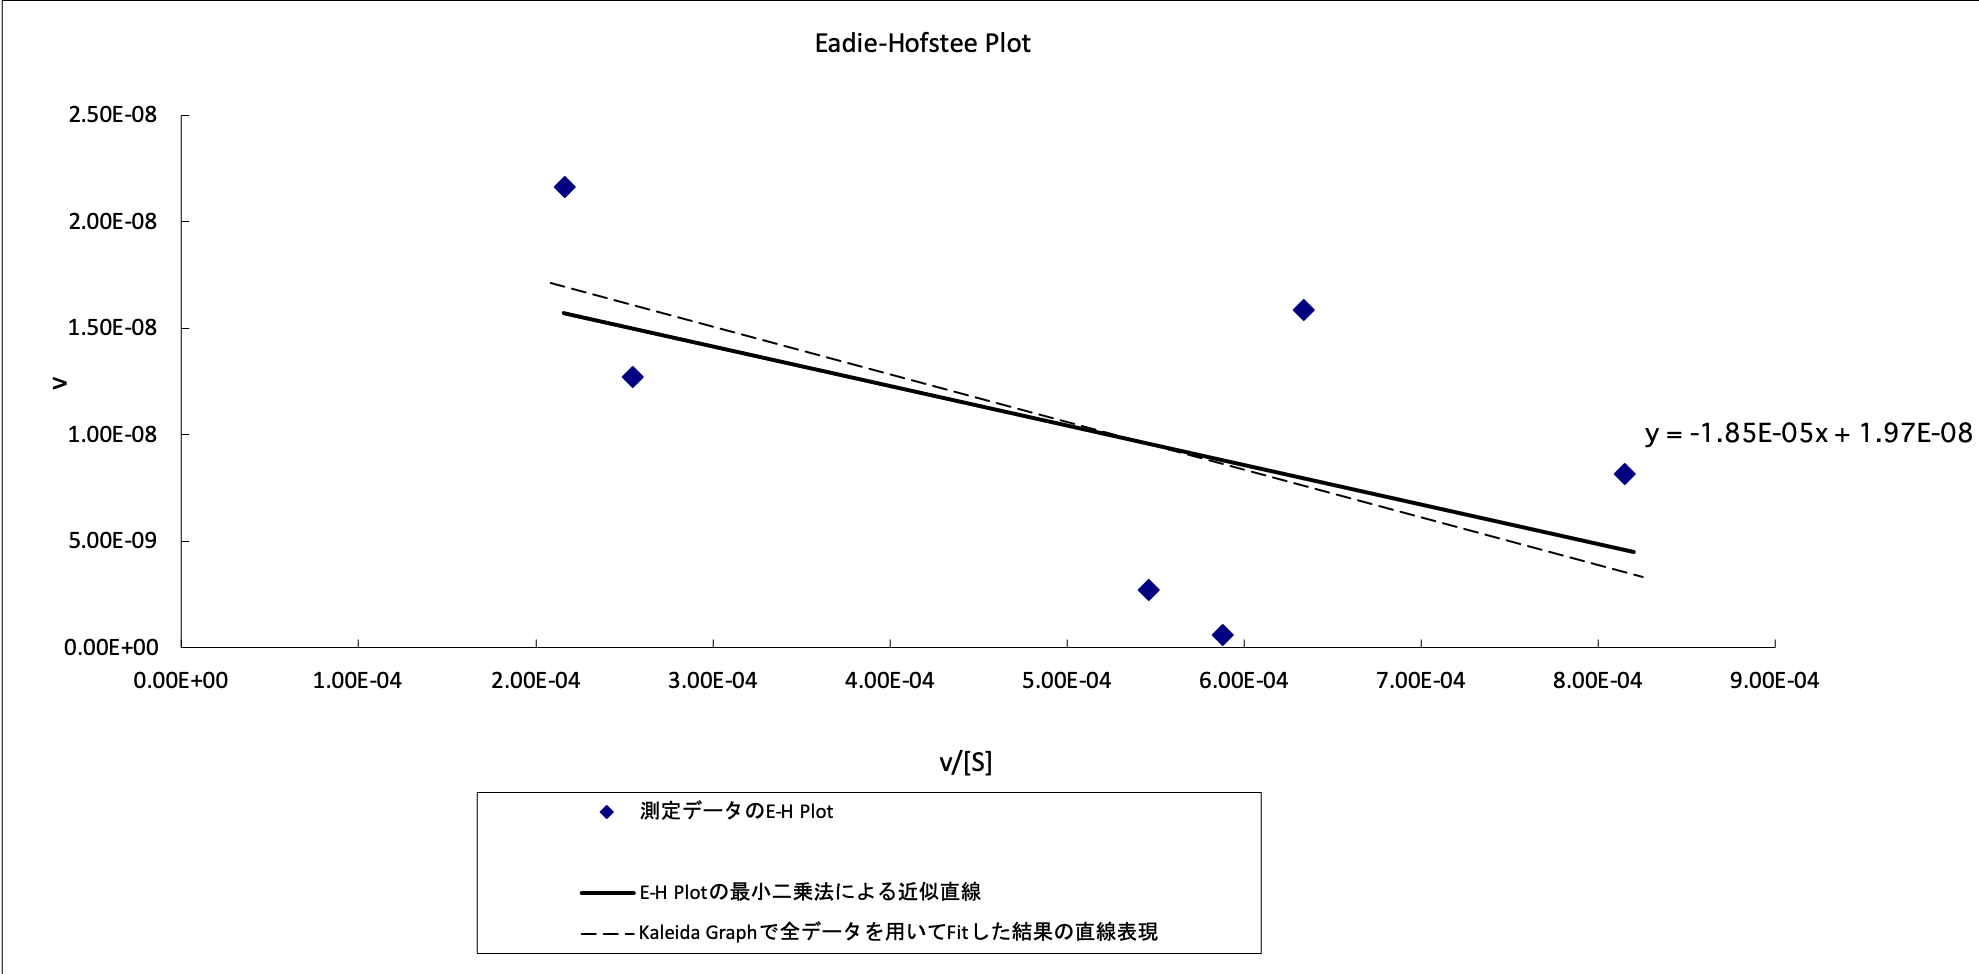
\includegraphics[clip, height=7cm]{imgs/11-eh.png}
\caption{L-B plot (実習)}
\end{center}
\end{figure}

\subsubsection*{5. それぞれの値の比較}
それぞれのプロットから算出された$k_{cat},
K_m,k_{cat}/K_m$について比較する。

\begin{table}[H]
\begin{center}
\begin{tabular}{|c|c|c|c|c|}
\hline
& M-M 6     & M-M 4     & L-B       & E-H       \\ \hline
$k_{cat} \ _{[s^{-1}]}$ & 6.125 & 18.725 & 23.025 & 4.925 \\ \hline
$K_m \ _{[\mu M]}$ & 22.53 & 103.5 & 49.71 & 20.85 \\ \hline
$k_{cat}/K_m \ _{[s^{-1} \cdot \mu M^{-1}]}$   & 0.2704 & 0.1979 & 0.1744 & 0.2538 \\ \hline
$\Sigma \epsilon i^2$    & $2.932 \times 10^{-5}$ & - & $1.679 \times 10^{-4}$ & $1.930 \times 10^{-4}$ \\ \hline
\end{tabular}
\caption{自作プログラムで得られたパラメータ}
\end{center}
\end{table}

\begin{table}[H]
\begin{center}
\begin{tabular}{|c|c|c|c|c|}
\hline
& M-M 6     & M-M 4     & L-B       & E-H       \\ \hline
$k_{cat} \ _{[s^{-1}]}$ & 6.091 & 20.49 & 8.668 & 5.293 \\ \hline
$K_m \ _{[\mu M]}$ & 22.8 & 92.7 & 155 & 18.5 \\ \hline
$k_{cat}/K_m \ _{[s^{-1} \cdot \mu M^{-1}]}$   & 0.267& 0.221 & 0.0559 & 0.286 \\ \hline
$\Sigma \epsilon i^2$    & $3.23 \times 10^{-5}$ & - & $3.18 \times 10^{-4}$ & $5.20 \times 10^{-5}$ \\ \hline
\end{tabular}
\caption{実習プログラムで得られたパラメータ}
\end{center}
\end{table}




\part*{実験3 細胞の状態に応じた酵素活性変化の測定}

\section*{目的}
細胞の状態に応じた酵素活性の変化を蛍光プローブを用いて検出する実験として、細胞のアポトーシスをともなうcaspase-3の活性化の検出を試みる。

\section*{実験方法}
UV照射によってアポトーシスを誘導したJuckat T細胞(アポトーシス群)とUV照射しないコントロール群の細胞の培養液各10 mLを遠心(2000rpm, 5min)し、上清を除いてPBS 3 mLで洗浄し、PBS 300 $\rm \mu L$を加えて超音波破砕によって細胞膜を破壊し、細胞ライセートとする。

PBSを用いて検量線用の0.2, 0.4 0.6 0.8 mg/mLのBSAの希釈系列を作成する。細胞ライセートを5倍希釈した試料を調整し、各サンプル(PBAのみ、BSA希釈系列、細胞ライセート5倍希釈(アポトーシス群、コントロール群)×3)を10 $\rm \mu L$ずつマルチウェルプレートに添加し、それぞれにbradford試薬200 $\rm \mu L$を添加して5分静置する。595 nmの吸収を測り、BSA希釈系列から検量線を作成して細胞ライセートのタンパク質濃度を算出する。

\section*{結果}

\begin{table}[H]
\begin{center}
\begin{tabular}{|c|c|c|c|c|c|}
\hline
BSA濃度 (mg/mL) & 0     & 0.2   & 0.4   & 0.6   & 0.8   \\ \hline
吸光度 & 0.317 & 0.293 & 0.438 & 0.505 & 0.581 \\ \hline
\end{tabular}
\end{center}
\end{table}

PBSのみの方がBSA濃度が0.2 mg/mLの時よりも吸光度が大きいので単調増加なプロットにはならなかった。

\pict{imgs/day4.png}{11}

また、細胞ライセートの吸光度は以下のようになった。

\begin{table}[H]
\begin{center}
\begin{tabular}{|c|c|c|c|c|}
\hline
 & 1 & 2 & 3 & Average \\ \hline
アポトーシス群 (mg/mL) & 0.427 & 0.489 & 0.493 & 0.470 \\ \hline
コントロール群  (mg/mL) & 0.577 & 0.535 & 0.596 & 0.569 \\ \hline
\end{tabular}
\end{center}
\end{table}

吸光度の平均値から各群の濃度を求めると以下のようになる。

\[\mbox{アポトーシス群} =  0.832 mg/mL\]
\[\mbox{コントロール群} =   1.37 mg/mL\]


また、さらにPBSで0.5 mg/mLになるように細胞ライセートを調整し、各200 $\rm \mu L$のアポトーシス群、コントロール群、PBSのみのサンプルに2 $\rm \mu L$の蛍光プローブ溶液(10mM)を加えて30分37℃でインキュベーションし、蛍光スペクトルを測定する。($\lambda _{ex.}=355 \  \rm{nm} \ ,\ \lambda_{em.}=460 \  \rm{nm}$)

計測された蛍光強度は以下のようになった。

\begin{table}[H]
\begin{center}
\begin{tabular}{|c|c|c|}
\hline
アポトーシス  & コントロール  & PBS     \\ \hline
977.865 & 122.696 & 183.218 \\ \hline
\end{tabular}
\end{center}
\end{table}

\newpage

\section*{課題(実験2,3共通)}

\begin{tcolorbox}[colback=white,colbacktitle=black,coltitle=white,title={1. }]
酵素反応の速度を議論する上での$k_{cat}/K_m$の意味を考えよ。
\end{tcolorbox}
ミカエリス・メンテン式より
\[v = \frac{V_{max}[S]}{K_m+[S]}\]
また、$V_{max}=k_{cat}  [E]_0$より
\[v = \frac{k_{cat}[E]_0[S]}{K_m+[S]}\]


$k_{cat}$は酵素1分子が単位時間にどれだけ触媒として働けるか、つまり酵素の回転効率を表すパラメータである。したがって、$k_{cat}$が大きいほど反応速度も大きくなる。

$K_m$は基質との親和性を表すパラメータであり、値が小さいほど基質との親和性が大きくなるため、反応速度も大きくなる。

ミカエリス・メンテン式において、$K_m >> [S]$が成り立つ条件では
\[v = \frac{k_{cat}}{K_m}[E]_0[S]\]
このように近似される。すなわち$k_{cat}/K_m$は基質濃度が低い条件での酵素と基質の二次反応における反応速度定数に等しい。


\[v= \frac{k_{cat}}{K_m}\]

\

\begin{tcolorbox}[colback=white,colbacktitle=black,coltitle=white,title={2. }]
TB-$\beta$GalとDAFの蛍光制御原理の共通点および違いについて説明せよ。
\end{tcolorbox}

本来蛍光団のLUMOからHOMOに電子が戻るときには電磁波が発せられるが、蛍光団のHOMOとLUMOの間のエネルギー準位に電子供与体のHOMOが存在すると、そこから蛍光団のHOMOに電子が供給される緩和過程があるために蛍光を発さなくなる。このメカニズムによって蛍光を制御しているのがTG-$\beta$GalとDAFの共通点である。

TG-$\beta$Galは、蛍光を持たないTG-$\beta$Galの状態と蛍光を示す2-Me-4OMe-TGの間で電子供与基に変化がない。TG-$\beta$Galの状態で電子供与基のHOMOは蛍光団のHOMOとLUMOの間にあるため蛍光を示さないが、$\beta$-galactosidaseによって加水分解されて2-Me-4-OMe-TGのアニオンの状態になると、蛍光団のHOMOのエネルギー準位が電子供与基のHOMOよりも高くなって蛍光を発するようになる。

それに対して、DAFは電子供与基が変化することで蛍光を制御している。電子供与基がジアミノベンゼンの状態の時は還元性が強く、HOMOのエネルギー準位が蛍光団のHOMOよりも高くないため蛍光を発さない。しかし、NOと反応してトリアゾール環構造となると電子供与基のHOMOのエネルギー準位が蛍光団のHOMOよりも低くなって蛍光を発するようになる。

\

\begin{tcolorbox}[colback=white,colbacktitle=black,coltitle=white,title={3.}]
 M-M Plot, L-B Plot , E-H Plot のずれはなぜ生じるのか。データ解析をする上でどのプロットが最も正確に実験結果を反映しているか。
\end{tcolorbox}

パラーメータをまとめた表は結果の項を参照して欲しい。

M-M plotは最小二乗法によって直接Michaelis-Mentenの式に最適化しているため誤差の二乗和の値が最も小さく、一番正確に実験結果を反映していると言える。
L-B plotとE-H plotを比べると、自分の作ったプログラムの結果ではL-B plot の方が誤差の二乗和が小さいが、実習で用いたプログラムの結果ではE-H plotの方が誤差の二乗和の値が小さい。
原理としてはL-B plotでは低濃度の逆数である1, 0.2, 0.1が他の値と大きく離れるために近似直線を引く上で大きなウエイトをもつが、逆に高濃度側ではx軸の値の差異が小さいため、近似直線に影響を与えにくい性質がある。そのため、高濃度部分で誤差が大きくなりやすい。
E-H plotはx軸に反応速度を基質濃度で割った値を用いることで、高濃度領域でも低濃度領域でも同じウエイトがかかるようになっている。そのためプロットのx座標が極端に偏らずに万遍なく分布する。そのため算出されるパラメータの誤差は小さくなると考えられる。

\

\begin{tcolorbox}[colback=white,colbacktitle=black,coltitle=white,title={4. }]
実習1で用いたBCA法、実習3で用いたBradford法の2つのタンパク質定量法の原理について述べよ。
\end{tcolorbox}

\subsubsection*{Bradford法}
Coomassie G-250を用いた総蛋白定量法である。Coomassie G-250は酸性条件下でタンパク質と結合して吸光が変化する。タンパク質と結合していない時としている時の吸光度の差が最も大きくなるのが595 nm付近であることから、一般的に595 nmで吸光度を測定する。
Bradford法のメリットとしては反応時間が短いことや還元剤や塩との共存性が高いことが挙げられる。一方で検量線の直線性が低いことや界面活性剤により反応が阻害されるという欠点もある。

\subsubsection*{BCA法}
BCA法は、アルカリ条件下でタンパク質によって$\rm Cu^{2+}$が$\rm Cu^+$に還元される原理と、$\rm Cu^+$が2分子のビシンコニン酸と配位結合して紫色に呈色する原理を組み合わせた方法である。
まずタンパク質と2価の銅イオン$\rm Cu^{2+}$がキレート錯体を形成するビューレット反応を起こす。ビューレット反応はアミノ酸では起きないがペプチド鎖が3つ以上であれば反応が起こり、540 nm付近に吸収のある複合体を形成する。
その後$\rm Cu^{2+}$がタンパク質によって$\rm Cu^+$に還元される。この$\rm Cu^+$が2分子のBCA試薬と紫色の錯体を形成する。
タンパク質の単位質量あたりに存在するペプチド結合の数はほぼ一定であるため、BCA/Cu+ 複合体の発色はタンパク質濃度に比例する。したがってBCA法では決定係数が0.95を超えるような非常に直線的な検量線が得られる。
BCA法はBradford法の弱点である界面活性剤との共存性が高いという利点があるが、逆に元剤や銅イオンのキレート剤により反応が阻害というデメリットがある。

\

\begin{tcolorbox}[colback=white,colbacktitle=black,coltitle=white,title={5.}]
 あなたが考える「蛍光プローブでしかできない実験」を簡単に述べよ。
\end{tcolorbox}

蛍光プローブは被験体となる生物が生きている状態で観察できるので、様々な動物実験に応用できる可能性がある。例えば、乳酸などの筋疲労によって生じる物質に対して特異的に蛍光する物質があれば、筋トレや有酸素運動の効き具合が定量的に確認できるかもしれない。

\

\begin{tcolorbox}[colback=white,colbacktitle=black,coltitle=white,title={6.}]
 実習1,2,3を通じての感想
\end{tcolorbox}

実習中は作業が多くて、今自分がしている作業の意味を理解していませんでしたが、実習を終えてレポートを書くことで、この作業はこういうことをしていたのかと再確認できました。それによって蛍光プローブの魅力が少しはわかったと思います。

それ以上に印象に残っているのがミカエリス・メンテン式などのプロットを行うプログラムを作成したことです。それぞれの関数、フィッティング方法を指定し、パラメーターの出力まで行うことで式の理解やパラメータのもつ意味を理解することができたと思います。

\end{document}